\smallskip

On considère $n$ un entier naturel non nul.

On considère la fonction $f_n$ définie sur l'intervalle $[0~;~1]$ par :
$f_n(x) = x^n \e^{1 - x}.$

\smallskip

\textbf{Partie A}

\smallskip

\begin{enumerate}
	\item  $f_1(x)=x \e^{1-x}$ donc $f'_{1}(x) = 1 \times \e^{1 - x} + x \times \left(-\e^{1-x}\right) = \boxed{(1-x)\e^{1-x}}$

On sait que pour tout $x \in \R$ on a $\e^{1-x} > 0$, donc $f'_{1}(x)$ est du signe de $1 - x$. Or, $1 - x \geqslant 0 \iff x \leqslant 1$. Donc, pour tout $x \in \intervFO{0}{1}$, $f'_{1}(x)$ est strictement positif.

	\item\
	
\begin{minipage}{.667\textwidth}
	\begin{center}
	\begin{tikzpicture}
		\tkzTabInit[lgt=2.5,espcl=3]{$x$/0.8,Signe de $f_{1}(x)$/1,Variations de $f_{1}$/2.5}{$0$,$1$}
		\tkzTabLine{,+,}
		\tkzTabVar{-/$0$,+/$1$}
		\end{tikzpicture}
	\end{center}
	\end{minipage}\hfill
	\begin{minipage}[t]{.275\textwidth}
	\[f_{1}(0) = 0 \times \e^{1-0} = 0\]
	\[f_{1}(1) = 1 \times \e^{1-1} = \e^{0} = 1\]
\end{minipage}

\smallskip

	\item La fonction $f_{1}$ est continue (puisque dérivable) et strictement croissante sur \intervFF{0}{1}, avec

$f_{1}(0) = 0 < 0,1$ et $f_{1}(1) = 1 > 0,1$, donc, d'après le corollaire du théorème des valeurs intermédiaires, l'équation $f_{1}(x) = 0,1$ admet une solution unique dans \intervFF{0}{1}.
\end{enumerate}

\smallskip

\textbf{Partie B}

\smallskip

On considère la suite $(u_n)$ définie pour tout entier naturel $n$ non nul par 

\begin{center}$u_n = \displaystyle\int_0^1 f_n(x) \:\text{d}x$ \quad  c'est-à-dire \quad $u_n = \displaystyle\int_0^1 x^n \e^{1-x} \: \text{d}x$.\end{center}

On admet que $u_1 = \e - 2$.

\begin{enumerate}
	\item 
	
	\begin{enumerate}
	\item 	Pour $x \in \, [0~;~1]$, on a: $0\leqslant x \leqslant 1$.

$x\geqslant 0$ donc $x^n\geqslant 0$; on multiplie l'inégalité précédente par $x^n$:

$0\times x^n \leqslant x \times x^n  \leqslant 1 \times x^n 
\iff 0 \leqslant x^{n+1} \leqslant x^n$
	
On a donc démontré que pour tout entier naturel $n$, on a:

\[\boxed{0 \leqslant x^{n+1} \leqslant x^n}\]


		\item On sait que pour tout $x \in \R$, $\e^{1-x} > 0$, donc, d'après la question précédente :

\[0 \leqslant x^{n+1} \leqslant x^{n} \iff 0 \leqslant x^{n+1}\e^{1-x} \leqslant x^{n}\e^{1-x}.\]
		
		Donc, d'après la positivité de l'intégration :

\[0 \leqslant x^{n+1}\e^{1-x} \leqslant x^{n}\e^{1-x} \implies 0 \leqslant \int_{0}^{1}x^{n+1}\e^{1-x}\d x \leqslant \int_{0}^{1}x^{n}\e^{1-x}\d x \iff \boxed{0 \leqslant u_{n+1} \leqslant u_{n}}\]

		\item D'après la question précédente, puisque $u_{n+1} \leqslant u_{n}$ la suite $\left(u_{n}\right)$ est décroissante.
		
De plus, puisque $0 \leqslant u_{n}$, elle est minorée par $0$. 

Donc, d'après le théorème de convergence monotone, la suite $\left(u_{n}\right)$ est convergente vers une limite positive ou nulle.
	\end{enumerate}
	
	\item
	\begin{enumerate}
		\item On sait que pour $u$ et $v$ dérivables on a : $\displaystyle\int_{a}^{b}u'(x)v(x)\d x = \left[u(x)v(x)\right]_{a}^{b} - \displaystyle\int_{a}^{b}u(x)v'(x)\d x$.

Posons $u'(x) = \e^{1-x}$ et $v(x) = x^{n+1}$. 
Alors $u(x) = -\e^{1-x}$ et $v'(x) = (n+1)x^{n}$. 

On a donc :

\begin{eqnarray*}
	\int_{0}^{1}x^{n+1}\e^{1-x}\d x &=& \left[-x^{n+1}\e^{1-x}\right]_{0}^{1} - \int_{0}^{1}(n+1)x^{n}\left(-\e^{1-x}\right)\d x\\
	&=& -1^{n+1}\e^{1-1} - \left(-0^{n+1}\e^{1-0}\right) - (n+1)\int_{0}^{1}-x^{n}\e^{1-x}\d x\\
	&=& -1 + (n+1)\int_{0}^{1}x^{n}\e^{1-x}\d x
\end{eqnarray*}

On a donc bien :

\[\boxed{u_{n+1} = (n+1)u_{n} - 1}.\]

\item On complète le script Python en bleu ci-dessus pour que la fonction \texttt{suite()} renvoie la valeur de $\displaystyle\int_0^1 x^8 \e^{1-x} \, \text{d}x$.

\begin{center}
\fbox{\parbox{.5\textwidth}{
\begin{ttfamily}
	from math import exp\\
	\\
	\begin{tabular}{ll}
def	& suite() :\\
	& u = \blue \textbf{exp(1)-2}\\
	& for n in range (1,{\blue\textbf{8}}):\\
	& \qquad u = \blue\textbf{(n+1) * u - 1}\\
	& return \blue u
	\end{tabular}
\end{ttfamily}}}
		\end{center}
	\end{enumerate}
	
\item
	\begin{enumerate}
		\item On se place dans l'intervalle d'intégration : soit $x \in [0~;~1]$, donc 













$\begin{aligned}[t]
0 \leqslant  x \leqslant 1 
 &\implies  1-x  \leqslant 1 
\implies   \e^{1-x} \leqslant \e \text{~~~~(croissance de la fonction exponentielle)}\\
 &\implies   x^n \e^{1-x} \leqslant x^n\times \e ~~~~(x^n\geqslant 0)\\
 &\implies   \ds\int_{0}^{1} x^n \e^{1-x} \d x \leqslant \ds\int_{0}^{1}   x^n\times \e \d x \text{~~~~(craoissance de l'intégration)}\\
 &\implies   \ds\int_{0}^{1} x^n \e^{1-x} \d x \leqslant \e \ds\int_{0}^{1} x^n \d x
\implies   u_n \leqslant \e \left [ \dfrac{x^{n+1}}{n+1} \right ]_{0}^{1}\\
 & \implies   u_n \leqslant \dfrac{\e}{n+1} \\
\end{aligned}$

\item On sait que pour tout $n$, on a: $0\leqslant u_n$; donc $0\leqslant u_n \leqslant \dfrac{\e}{n+1}$.

Or  $\displaystyle\lim_{n \to + \infty} \dfrac{\e}{n+1} = 0$, donc d'après le théorème des gendarmes, on peut dire que  

\[\boxed{\displaystyle\lim_{n \to + \infty} u_n = 0}\]
	\end{enumerate}
\end{enumerate}


\bigskip
